\clearpage
\subsection{ツェナーダイオードの特性実験}
\subsubsection{ツェナーダイオードの実験器具}
使用した実験器具を\wtab{kigu2}に示す.
\begin{table}[h]
  \centering
  \caption{実験装置}
  \label{tab:kigu2}
  \scalebox{1.0}{
  \begin{tabular}{cccccc}
    \hline
    機器名&製造元&型番&シリアル番号(または管理番号)\\
    \hline
    ダイオード&不明&1N4736A&不明\\
    直流電源&YOKOGAWA&PA1811&L96-000668\\
    直流用電圧計&YOKOGAWA&YAS 1991&71 BA0 3371\\
    ミリアンペア直流用電流計&YOKOGAWA&YES 1990&70 BA0 1812\\
    \hline
  \end{tabular}
}
\end{table}

\subsubsection{ツェナーダイオードの実験方法}
\begin{enumerate}[(1)]
\item \wfig{zenerc}のように回路を構築する.なお,電圧計は$10\,\rm{V}$端子,電流計は$30\,\rm{mA}$端子に接続して計測を行った.また,配線時にダイオードの向きに注意する必要がある.
\item $V_{i}$を$0\,\rm{V}$から$18\,\rm{V}$まで$0.1\,\rm{V}$刻みで増加させ,電流$I_{Z}$と電圧$V_{L}$を計測する.
\item 上記で計測したデータをもとに,$V_{i}-V_{L}$特性,$V_{i}-I_{Z}$を同一グラフに描画した.
\begin{figure}[h]
\centering
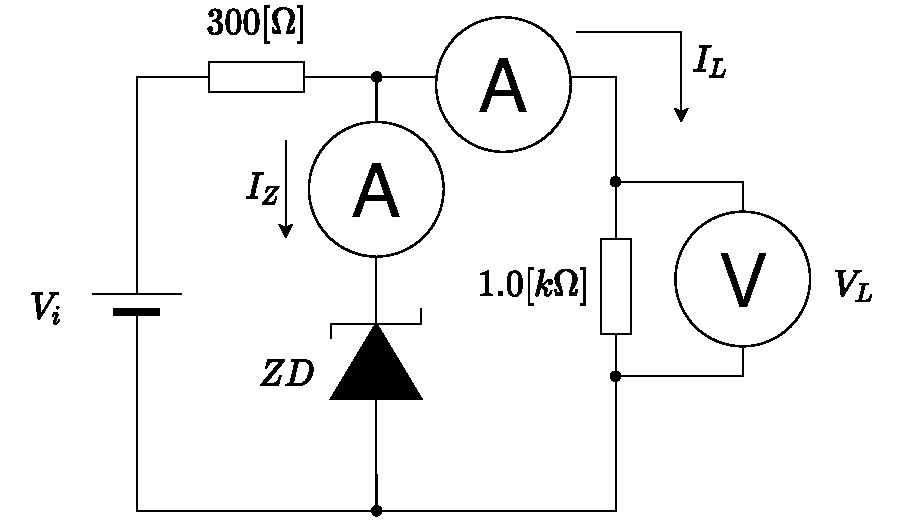
\includegraphics[scale=0.7]{./fig/zenerc.pdf}
\caption{ツェナーダイオード測定回路}
\label{fig:zenerc}
\end{figure}
\end{enumerate}

\subsubsection{ツェナーダイオードの結果}
\begin{itemize}
\item \wtab{zener-tab}に測定したデータをまとめた.
出力電圧が$10\,\rm{V}$付近からツェナー電流の増加が起きていることがわかる.
また,出力電圧$V_{L}$は$8\,\rm{V}$以降,入力電圧が増加してもあまり変化が起きていない.
\item \wfig{zenerg}は$V_{i}-V_{L}$特性,$V_{i}-I_{Z}$特性のグラフである.$V_{L}$は増加した後,ほぼ一定となっているのに対し,$I_{Z}$はほぼ一定($=0$)の後,増加と逆の動きをしている.
\begin{table}[h]
\centering
\caption{ツェナーダイオードの特性}
\label{tab:zener-tab}
\scalebox{0.9}{
\begin{tabular}{ccc}
\hline
入力電圧$V_i$$[\rm{V}]$ & 出力電圧$V_L$$[\rm{V}]$ & ツェナー電流$I_Z$$[\rm{mA}]$ \\
\hline
0    & 0.0       & 0.0      \\
1    & 0.8     & 0.0       \\
2    & 1.5       & 0.0          \\
3    & 2.3         & 0.0              \\
4    & 3.0           & 0.0              \\
5    & 3.8         & 0.0              \\
6    & 4.6         & 0.0           \\
7    & 5.3         & 0.0              \\
8    & 6.1         & 0.0           \\
9    & 6.8         & 0.1       \\
10   & 6.9         & 3.0           \\
11   & 6.9         & 6.2          \\
12   & 7.0           & 9.6           \\
13   & 7.0           & 12.8           \\
14   & 7.0           & 16.1           \\
15   & 7.0           & 19.4           \\
16   & 7.1         & 22.6        \\
17   & 7.1         & 25.9           \\
18   & 7.2      & 29.2     \\
\hline
\end{tabular}
}
\end{table}
\begin{figure}[h]
\centering
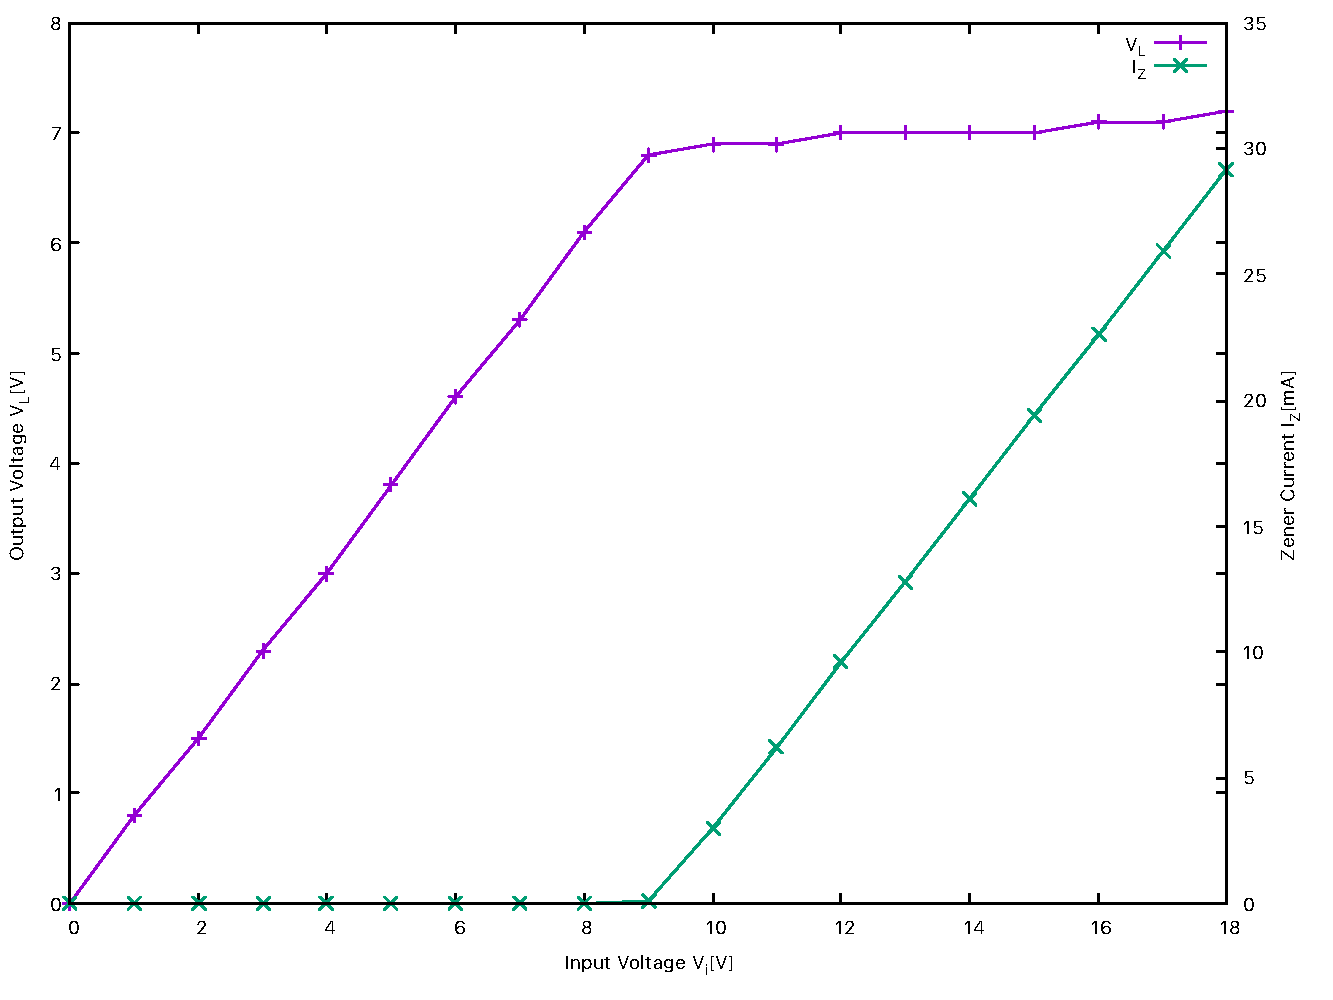
\includegraphics[scale=0.65]{./data/zener/zener-graph.pdf}
\caption{ツェナーダイオードの特性}
\label{fig:zenerg}
\end{figure}
\end{itemize}

\clearpage
\subsubsection{ツェナーダイオードの考察}
\begin{enumerate}[(1)]
\item 今回用いたツェナーダイオード1N4736Aをダイオード規格表(または,データシート)でツェナー電圧を調べ,実験結果と比較して考察せよ.

データシート~\cite{fbklsdn}を参照すると平均値は$6.8\,\rm{V}$($25^{\circ}$C)である.一方,実験結果より,ツェナー電圧は$6.8\,\rm{V}$から$7.2\,\rm{V}$で推移しており,データシートとの差異がほとんどなく,正しく計測できたといえる.
\item ツェナーダイオードはどういった場合に用いられるか説明せよ.

ツェナーダイオードは\wfig{diode-vi-curve-03}からわかるように,逆電圧を一定(降伏電圧, $V_{R}$)以上かけると急激に電流が流れるようになる特性がある.
この降伏電圧付近では,電流の広い範囲にわたって電圧が一定である.
すなわち,ダイオードに流れる電流の大きさに依存せずダイオードの電圧は一定に保たれるため.定電圧源として利用される\cite{1130282271098203vsdv4}.
\begin{figure}[h]
\centering
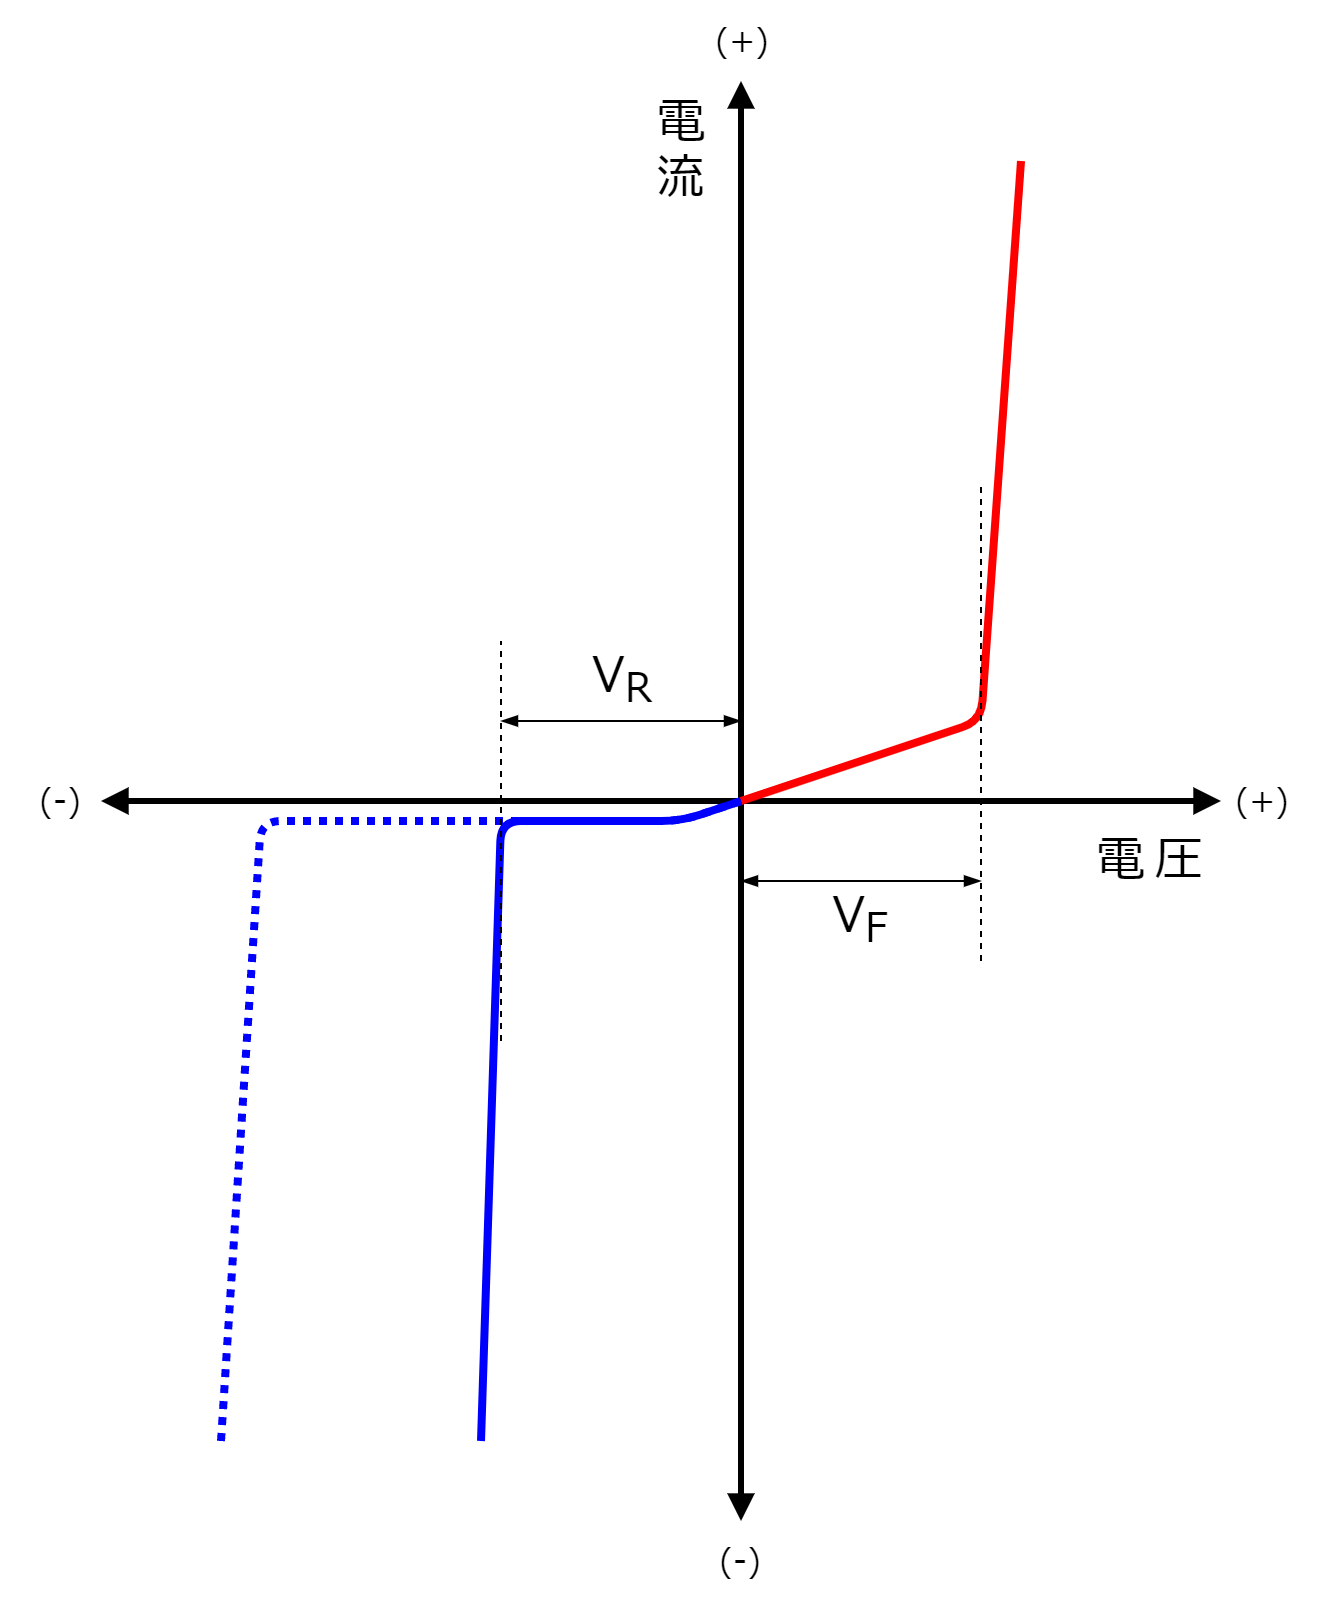
\includegraphics[scale=0.15]{./fig/diode-vi-curve-03.png}
\caption{ツェナーダイオードの特性図\cite{sdjabcklds}}
\label{fig:diode-vi-curve-03}
\end{figure}
\item  $V_{Z}-I_{Z}$特性のグラフを描き,ツェナー電圧$V_{Z}$を明記せよ.

\wfig{zener-v-i}に$V_{Z}-I_{Z}$特性を示す.なお,$V_{Z}$は$6.8\,\rm{V}$とした.
出力電圧はほぼツェナー電圧に近似できているが,実験結果と誤差が少し発生している.
\begin{figure}[h]
\centering
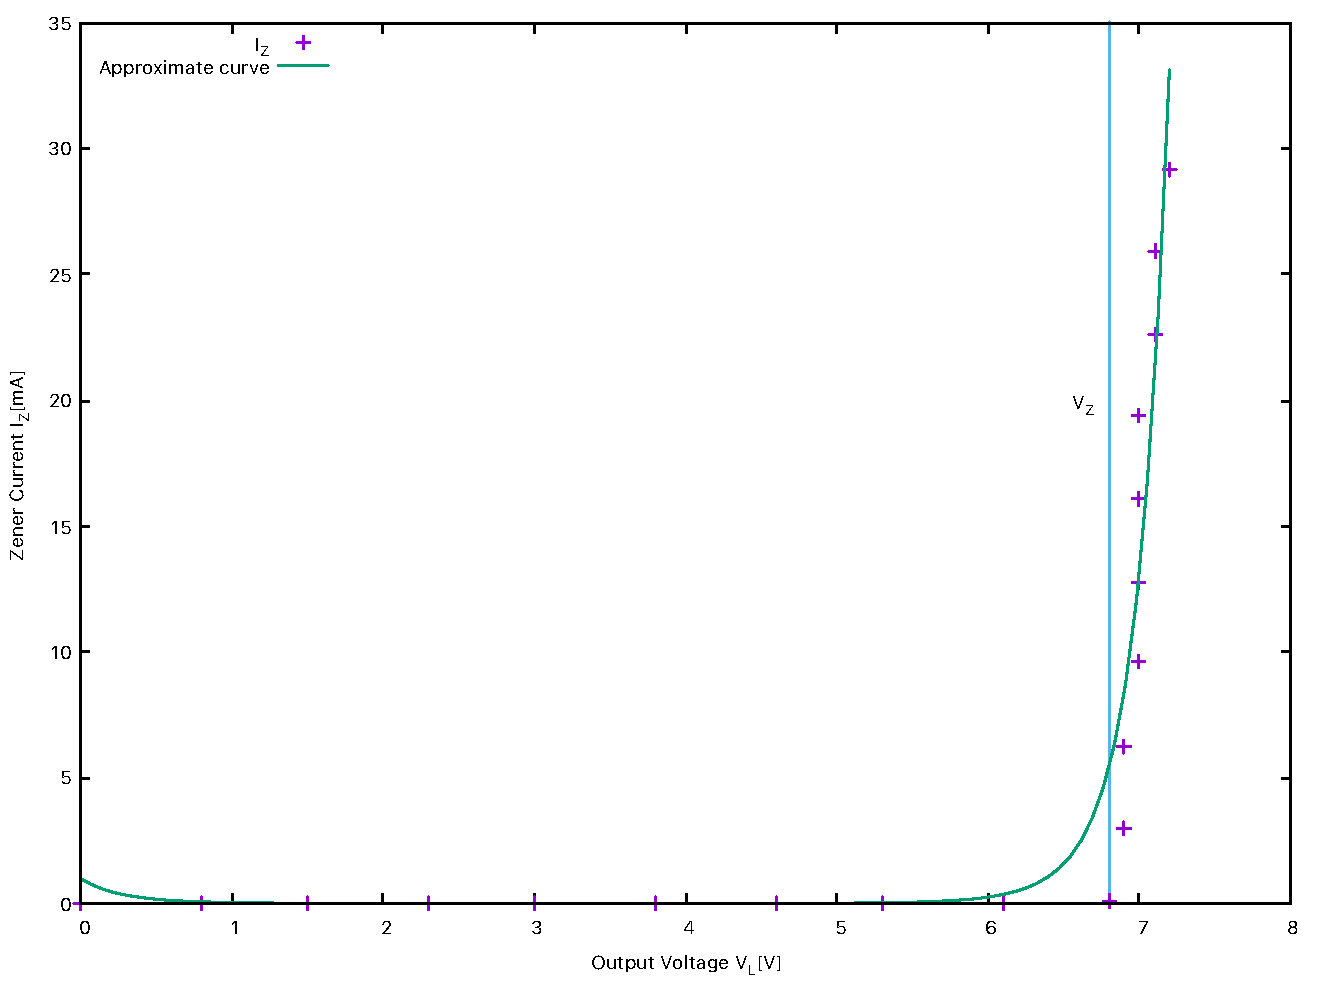
\includegraphics[scale=0.7]{./data/zener/zener-v-i.pdf}
\caption{ツェナーダイオードの特性}
\label{fig:zener-v-i}
\end{figure}
\item 各グラフから入出力特性を考察せよ.

入力特性($V_{i}-I_{Z}$)について考える.\\
\wfig{zenerg}より,立ち上がり電圧$V_{F}$は$0.9\,\rm{V}$で,以降$I_{Z}$は$V_{i}$とほぼ比例して増加している.その傾きは約$33\times 10^{-3}\,\rm{S}$である.\\
次に出力特性($V_{L}-I_{Z}$)について考える.\\
\wfig{zener-v-i}より,$V_{Z}$以降,急激に電流を通すようになる.そしてその時の電圧は$6.8\,\rm{V}$から$7.3\,\rm{V}$に落ちついている.
\end{enumerate}
